\section{Woche 4 - AK OpenSource \headerand OpenSource Forum Erfurt} \label{sec:bericht-wo-4}

% Woche 4 (2023-09-25 bis 2023-09-29)

\lweekdaymarginpar{Montag}

Geschlafen hatte ich nicht viel, da ich noch in die Nacht hinein an dem Skript für Dienstag gearbeitet hatte.
Mit meinem Chef bin ich noch einmal die Präsentation durchgegangen und konnte meine vielen inhaltlichen und organisatorischen Fragen stellen.
Mein Hauptproblem war das folgende: Mit dem Thema, wie wir unsere Software-Inventare aufbauen, hatte ich bisher nur wenige Berührungspunkte, sollte es aber in der Präsentation ansprechen.
Mein Chef hat sich dann dazu bereiterklärt, diesen Teil in der Präsentation zu übernehmen, da die verbleibende Zeit nicht reichen würden, in dieses Thema richtig einzusteigen.

Lange war ich jedoch nicht im Büro, da ich die Vorbereitung lieber zu Hause abschließen wollte, wo ich ungestört üben konnte.
Den Abend habe ich also genau damit verbracht, und damit, mein Gepäck für die morgige Reise zu packen.

\sweekdaymarginpar{Dienstag}

Am Dienstagmorgen starteten wir direkt vom Heidelberger Hauptbahnhof mit dem ICE nach Erfurt, die Reise verlief zum Glück ohne Komplikationen.
In einem eigenen Abteil besprachen mein Chef und ich noch einmal unsere Präsentation und haben sie noch einmal probeweise vorgetragen.

Nach unserer Ankunft in Erfurt ging es direkt zu den Räumlichkeiten der DB Systel.
Dort gab es zunächst einige einleitende Worte und eine Vorstandswahl, bevor ich mit meiner Präsentation dran war.
Obwohl ich bis etwa 15 Minuten vor Beginn der Präsentation noch relativ entspannt war, stieg meine Aufregung dann doch noch etwas.
Aber eigentlich gab es keinen Grund für die Aufregung:
Ich war gut vorbereitet, hatte die Präsentation mehrfach vorgetragen und die Themen, die ich vorstellen wollte, gehören zu meinem täglichen Arbeitsbereich seit drei Jahren.
Aber auch meine Kollegen vor Ort haben mich ermutigt und bisher hatte ich einen positiven Eindruck von den restlichen Anwesenden.

Wegen all dieser Umstände verlief die Präsentation sehr gut, ich konnte sie ohne Notizen vortragen und habe alles gesagt, was ich sagen wollte.
In der Mittagspause nach der Fragerunde habe ich mich noch weiter mit anderen Teilnehmern unterhalten können, die mir zu einer sehr interessanten und inhaltsgefüllten Präsentation gratulieren wollten.
Das hat mich natürlich sehr gefreut und da wurde mir klar, dass es eine gute Präsentation war.
Natürlich haben wir uns auch fachlich noch miteinander ausgetauscht und weitere Präsentationen über diverse Themen rund um Communities im Kontext OpenSource angehört.

Abends haben wir zusammen noch an einer Stadtführung und einem gemeinsamen Abendessen mit anderen Teilnehmern des OpenSource Forums des nächsten Tages teilgenommen.

\sweekdaymarginpar{Mittwoch}

Das eigentliche OpenSource Forum der {\bitkom} war dann der entspanntere Teil der Geschäftsreise.
Hier gab es den Tag lang drei unterschiedliche Präsentations-Tracks zu unterschiedlichen Themen, die man sich anhören konnte.
Ein großer Programmpunkt war auch der {\bitkom} OpenSource Monitor\footnote{\url{https://www.bitkom.org/opensourcemonitor2023}}, den die {\metaeffekt} gesponsert hat und damit einen Beitrag über den Cyber Resilience Act\footnote{\url{https://digital-strategy.ec.europa.eu/en/policies/cyber-resilience-act}} in diesem verfassen durfte.

\begin{figure}[htbp] % here, top, bottom, separate page
    \centering
    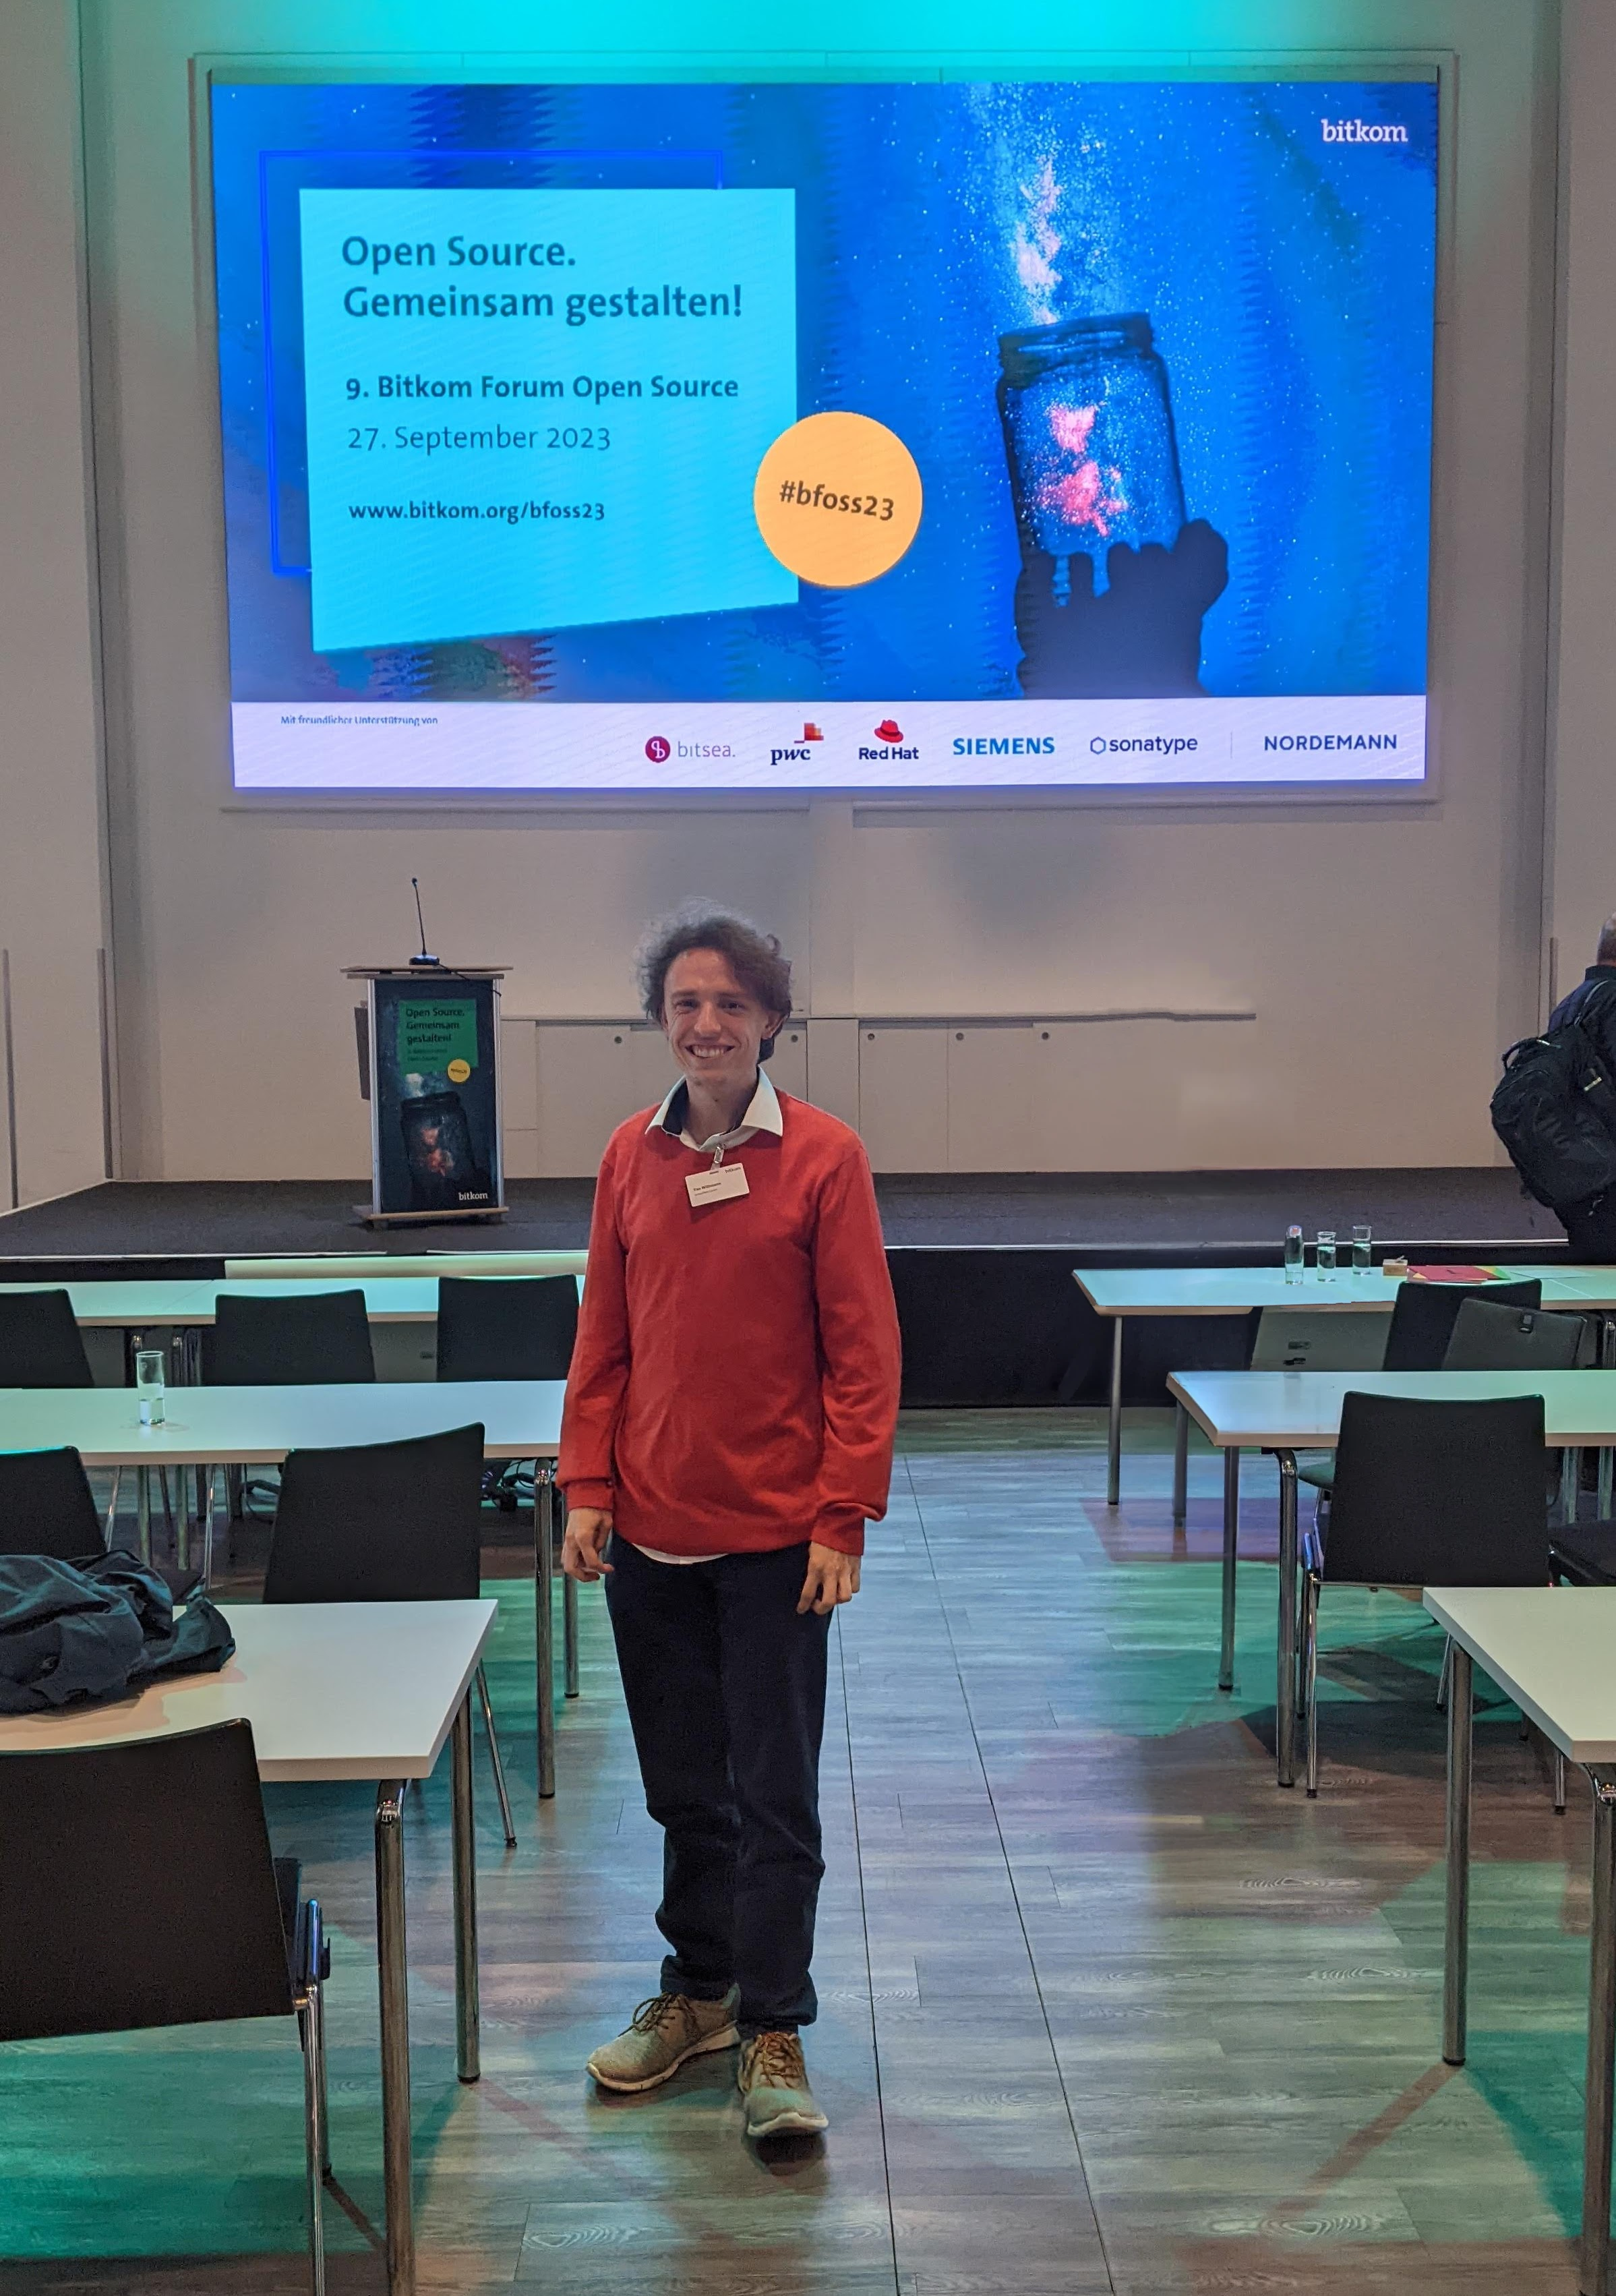
\includegraphics[width=0.5\textwidth, keepaspectratio]{res/img/2023-10-19-yan-ak-os}
    \caption{Auf dem Forum Open Source der {\bitkom} 2023}
    \label{fig:yan-foss23}
\end{figure}

Die Präsentationen waren sehr interessant zu hören, da sie von großen Unternehmen wie SAP, Siemens und Mercedes gehalten wurden und über ihre Probleme und Lösungen über die Verwaltung von Schwachstellen und Lizenzen von Open-Source-Software in ihren Produkten berichtet haben.
Das interessante war: Die ganzen Schritte, die alle diese Firmen im Moment durchlaufen, kommen uns sehr bekannt vor, denn an genau diesen Themen arbeiten wir bereits seit Jahren und entwickeln Lösungen dafür.

Natürlich gab es auch Pausen, in denen Teilnehmer miteinander networken konnten, was wir auch gut genutzt haben.
Es gab einige bekannte Gesichter vom vorherigen Tag, aber auch einige unserer Kunden waren vertreten, die ich noch nie in Person getroffen hatte.
Außerdem hatte ich die fantastische Chance direkt mit Studenten und Angestellten verschiedener Unterehen zu sprechen.

\sweekdaymarginpar{Do, Fr}

Donnerstag war mit der Heimreise gefüllt, an diesem Tag hatte ich nicht mehr gearbeitet.

Freitag ging es allerdings wieder ganz normal weiter im Geschäft.
Es ist wieder einmal eine neue Anforderung von einem Kunden in der Zwischenzeit hereingekommen:
Einer unserer Download-Prozesse scheitert bei ihm, da der verwendete git-Befehl die konfigurierte Proxy-Informationen im Moment noch ignoriert.

Die Herausforderung hier war, dass es sich im Gegensatz zu anderen download-Prozessen um einen tatsächlichen Zugriff auf einen lokalen Befehl handelt.
Git kann sowohl über Umgebungsvariablen konfiguriert werden, als auch über einen Konfigurationsstring im Befehlsaufruf.
Ich habe das Problem dann so gelöst, dass ich der Umgebung für die eine Prozess-Session, die über Java geöffnet wird, die entsprechenden Proxy-Informationen setze.

An diesem Freitag ist jedoch noch etwas Wichtigeres passiert, was zwar nicht unbedingt mit meinem Praktikum zu tun hat, aber dennoch mit mir als Person:
Mein Bruder hatte sich für eine Stelle beworben, die gerade freigeworden ist.
Da der vorherige Kollege auch nur ein anderer Student war, kann mein Bruder diese Arbeit auch ohne Informatikkenntnisse bewältigen.
Er war dann bei dem Weekly dabei, bei dem wir auch von unserem Ausflug nach Erfurt berichteten.
Er hat an diesem Tag noch den Arbeitsvertrag unterzeichnet und wird nun ebenfalls bei der {\metaeffekt} arbeiten.
